\subsection{Secunciación das actividades}
%• Desenvolvemento completo das diferentes sesións de clase, incluídos os anexos co material completo e necesario para aplicar a unidade didáctica.

As actividades constitúen unidades de traballo dentro da nosa unidade didáctica. De seguido amósanse as actividades que se levaron a cabo durante esta proposta didáctica.

En paralelo as actividades que imos describir a continuación fomos actualizando un sitio web creado a tal propósito e que se pode visitar en \href{http://leirasmates.ga}{leirasmates.ga}. Neste blogue publicamos os contidos que se explicaron durante a clase e incorporamos fontes de información adicionais como poden ser vídeos de YouTube onde se explican os mesmos contidos de forma diferente ou artigos de outras páxinas web. No Apéndice~\ref{fich:blogue} pódense ver as entradas que se publicaron neste blogue.

\subsubsection{Act. 0: Fotografando a xeometría}\label{act0}

Propoñeremos esta actividade como unha tarefa que o alumnado deberá realizar na casa. Trátase dunha actividade introdutoria na que o alumnado deberá enviar por correo electrónico fotografías con elementos xeométrico que poidan atopar na súa contorna. Entregarémoslles unha ficha que se pode ver no  Apéndice~\ref{fich:act0} coas instrucións da actividade. Nesta ficha pedimos que busquen fotos onde saian dúas rectas paralelas, dúas rectas que non o sexan (secantes), un polígono de 3 lados (un triángulo), un polígono de 4 lados (un cuadrilátero), un polígono de 5 lados ou máis e dun círculo.

O obxectivo desta actividade é que as alumnas e alumnos tomen conciencia de que está rodeados de obxectos matemáticos e ao mesmo tempo obter material co que poder traballar tanto para a posición relativa de rectas como para a clasificación de polígonos.

\begin{figure}[h!]
  \centering
  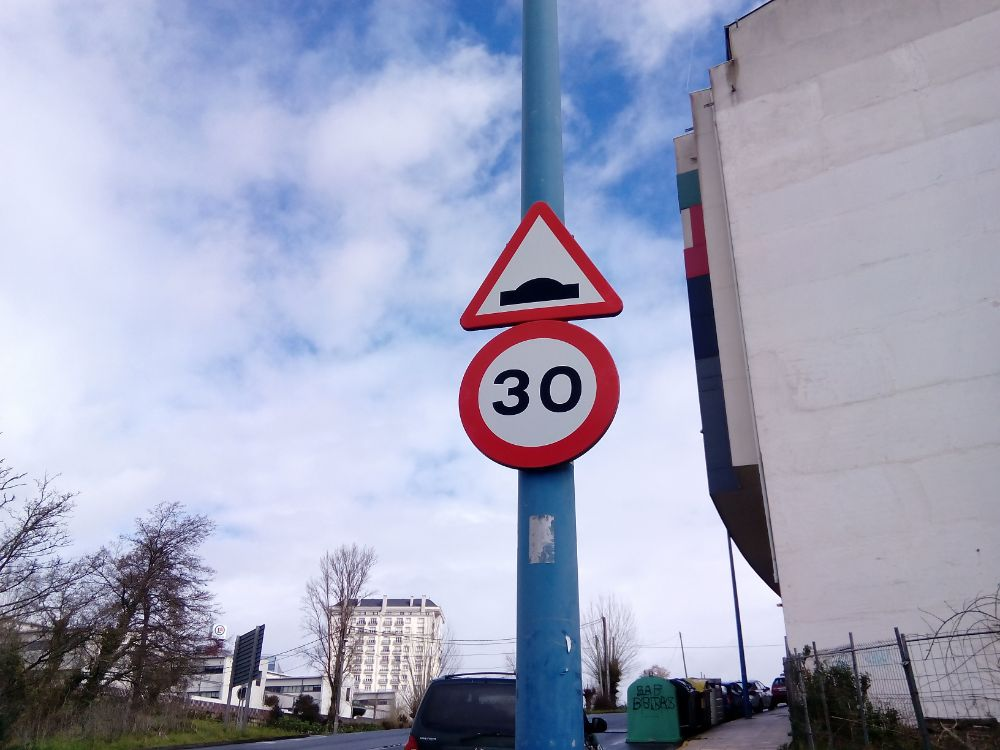
\includegraphics[height=4cm]{img/act0-1.jpg}
  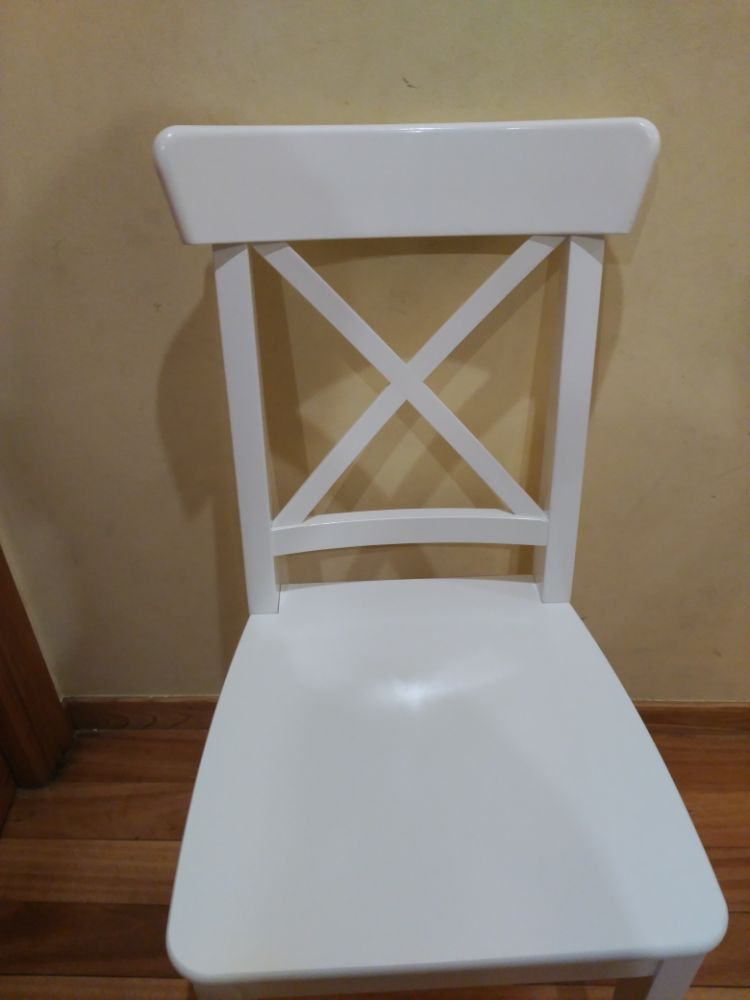
\includegraphics[height=4cm]{img/act0-2.jpg}
  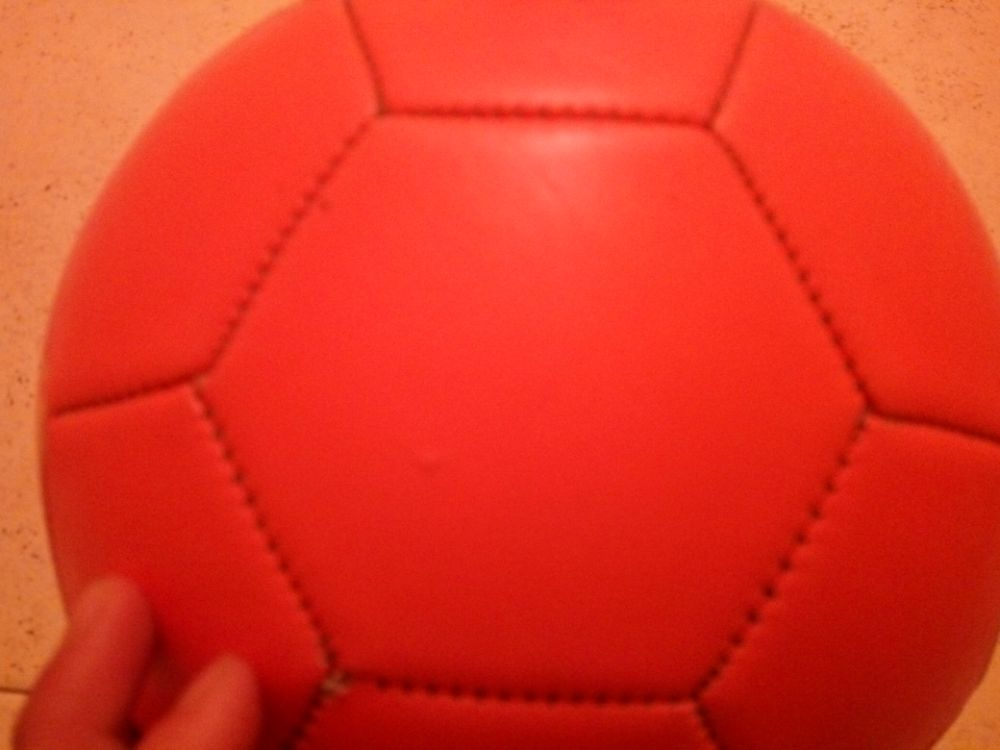
\includegraphics[height=4cm]{img/act0-3.jpg}
  \caption{Imaxes enviadas polos alumnos para a primeira actividade.}\label{fig:act0}
\end{figure}

Todas as fotos enviadas polo alumando serán subidas a web da materia. Na Figura~\ref{fig:act0} pódese ver algún exemplo do tipo de fotos que se buscan.

\subsubsection{Act. 1: Xeometría}
Como primeira activade do bloque de xeometría realizamos esta breve actividade introdutoria que pretende introducir ao alumnado no mundo da xeometría a par que se intenta habitualos nunha nova dinámica de clase na que se buscan a interacción docente-discente. Para introducilos no mundo da xeometría pedimos que definan coas súas palabras o que é a xeometría e a continuación mandarlles buscar por internet definicións de xeometría para que sexan lidas en voz alta. Para a realización desta actividade gastaremos sobre 10 minutos.

\subsubsection{Act.2: Puntos, liñas e posición relativa de liñas}\label{act2}
Durante esta actividade empezamos a explicar os elementos básicos de xeometría. Para facer isto comezamos preguntándolle aos alumnos e alumnas cal é para eles o elemento da xeometría máis simple que poden dicir. A raíz desta pregunta explicamos o concepto de punto. A raíz do punto explicamos que aliñando puntos obtemos unha recta. Explicase empregando un exemplo do programa Geogebra que a recta é infinita e que polo tanto non ten principio nin fin. A continuación expoñemos como se constrúe unha semirrecta, un segmento e detallamos a clasificación de rectas en función da súa posición relativa.

Para practicar a posición relativa das rectas realizamos unha actividade coas fotos de elementos xeométricos que enviaron na Actividade 0 (Sección~\ref{act0}). Durante esta actividade dividimos ha clase en grupos e cada grupo debe sinalar nas fotografías as rectas que sexan perpendiculares, secantes e paralelas. Para sinalar as rectas empregarase o programa de edición fotográfica, como pode ser GIMP.

\begin{figure}[h!]
  \centering
  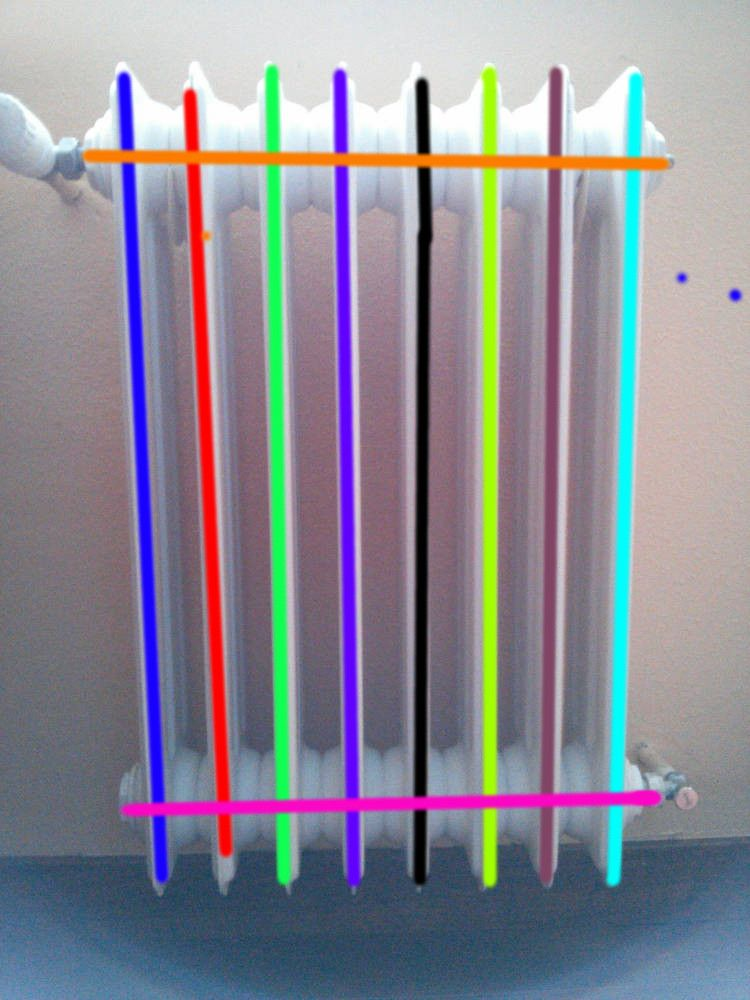
\includegraphics[height=4cm]{img/act1-img.jpg}
  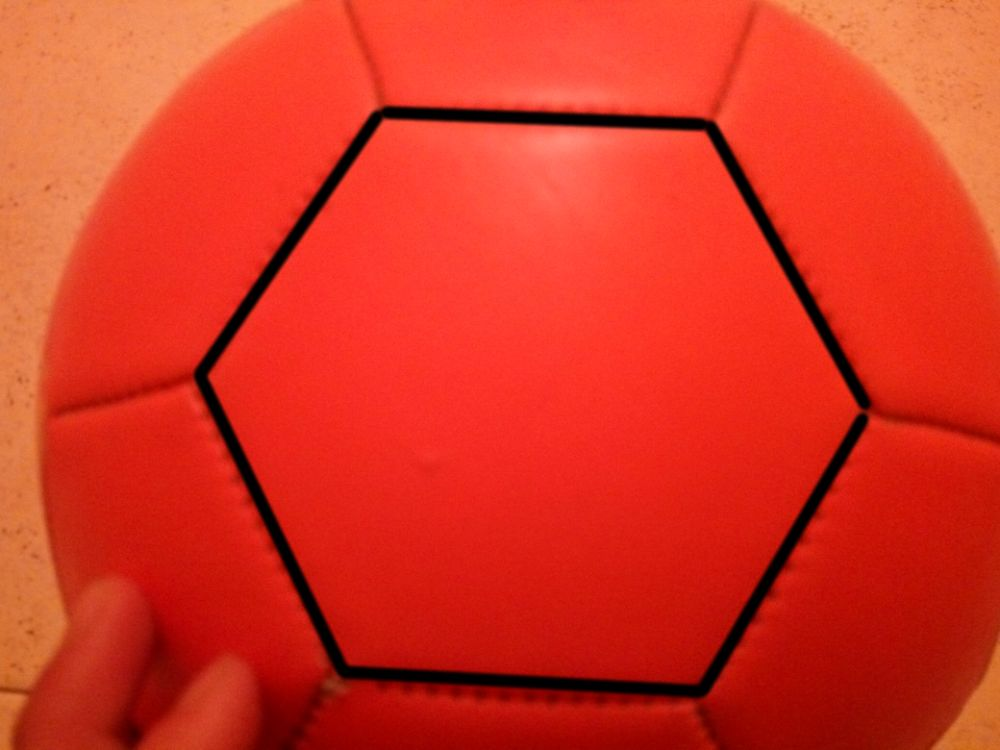
\includegraphics[height=4cm]{img/act1-img2.jpg}
  \caption{Marcado das imaxes con liñas paralelas, secantes e perpendiculares}\label{fig:act2}
\end{figure}

Despois de debuxar as rectas, os ficheiros son gardados e enviados por correo electrónico para ser proxectadas na clase. Cada grupo deberá explicar porque as rectas seleccionadoras teñen unha clasificación ou outra. Na Figura~\ref{fig:act2} pódense ver exemplos do que se pretende acadar. Dedicaremos a esta actividade aproximadamente 40 minutos.

\subsubsection{Act. 3: Ángulos e a súa clasificación}\label{act3}
Durante esta actividade explicaremos que é un ángulo así como a súa clasificación en función da súa amplitude e en función da súa posición relativa. Para practicar a clasificación de ángulos faremos un pequeno xogo onde as e os estudantes deberán por grupos clasificar diversos ángulos xerados aleatoriamente pola web \href{http://random.org}{Random.org}. Na Figura~\ref{fig:act5} pódese ver unha captura de pantalla dun ángulo xerado por esta web.

\begin{figure}[h!]
  \centering
  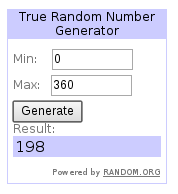
\includegraphics[height=5cm]{img/random.png}
  \caption{Captura de pantalla dun ángulo xerado por Random.org.}\label{fig:act5}
\end{figure}

\subsubsection{Act. 4: Sistema sexasesimal} %TODO
Explicamos o sistema sesaxesimal e como facer sumas e restas de grados expresados neste sistema. Baseamos a nosa explicación con unha comparación con algo que xa coñecen, a relación entre horas, minutos e segundos. Facemos varios exercicios propostos polo libro de texto sobre este tema.

\subsubsection{Act. 5: Mediatriz e bisectriz} %TODO
Explicamos os conceptos de mediatriz e de bisectriz e de como se trazan. Intentamos incidir nas propiedades que teñen a mediatriz e da bisectriz, e dicir, que os puntos destas dúas rectas equidistan dos extremos do segmento e dos lados do ángulo respectivamente. Estas propiedades serannos útiles máis tarde para explicar outros obxectos xeométricos como os puntos notables dos triángulos.

\subsubsection{Act. 6: Exame de xeometría básica}
Facemos un exame do explicado ata o momento que abrangue os conceptos de punto, rectas, planos, posición relativa de rectas, ángulos, clasificación de ángulos e posición relativa dos mesmos, sistema sesaxesimal, mediatrices e bisectrices. O exame que puxemos pódese ver no Apéndice~\ref{fich:ex1a}.

Intentando dar unha retroalimentación con respecto ao que o alumnado realizou neste exame o máis rápida posible corrixiremos os exercicios durante esa tarde e no día seguinte explicaremos todos os exercicios, os criterios de corrección e ensinámoslles ás alumnas e alumnos os exames corrixidos.

\subsubsection{Act. 7: Polígonos, triángulos e as súas clasificacións}\label{act7}
Expoñemos os conceptos de liña poligonal, de polígono e as clasificacións de polígonos en función dos seus ángulos e do número de lados. A continuación explicamos a clasificación dos triángulos en función dos seus ángulos e do número de lados iguais.

\begin{figure}[h!]
  \centering
  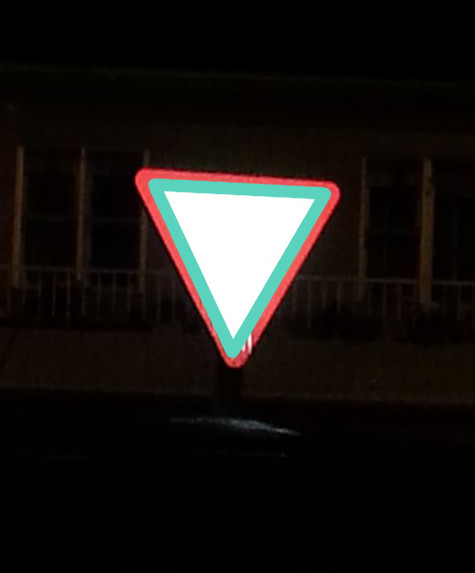
\includegraphics[height=5cm]{img/trian1.jpg}
  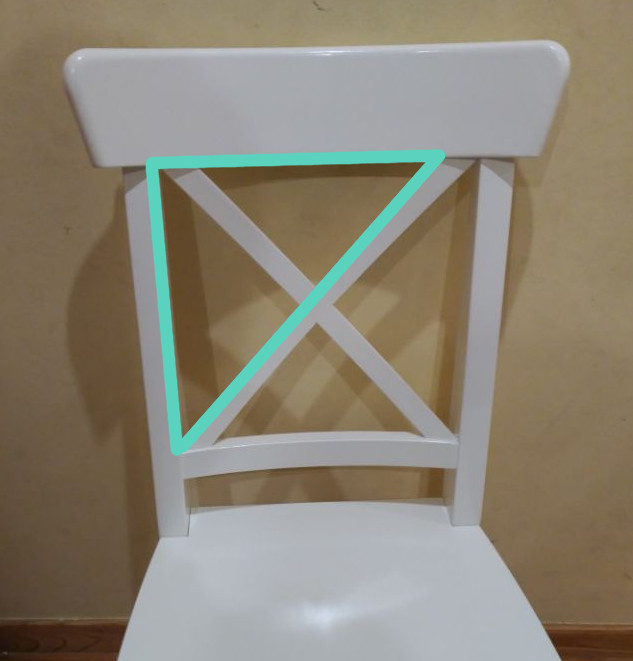
\includegraphics[height=5cm]{img/trian2.jpg}
  \caption{Exemplo de triángulo marcados sobre as fotografías}\label{fig:act7}
\end{figure}

Para practicar a clasificación dos triángulos realizamos un exercicio coas fotos que entregaron os alumnos durante a Actividade 0 (Sección~\ref{act0}). Para elo dividiremos a clase en grupos de 2 ou 3 persoas e cada grupo con un ordenador deberá buscar 4 triángulos diferentes nas fotos enviadas polos compañeiros. Da mesma forma que na segunda actividade, o alumnado deberá enviar as fotos editadas cos triángulos marcados ao ordenador do profesor no que se proxectarán. Cada grupo saíra e explicará a clasificación de cada un dos triángulos que marcou. Na Figura~\ref{fig:act7} pódense ver algúns exemplos das figuras que se pretenden acadar neste exercicio.

\subsubsection{Act. 8: Suma dos ángulos dun triángulo}\label{sec:sumang}
Nesta pequena actividade explicaremos e demostraremos de forma gráfica que a suma dos ángulos dun triángulo da sempre 180 grados. Para iso unha vez explicada esta propiedade na encerado, repartiremos triángulos feitos con goma-eva pero que, como se pode ver na Figura~\ref{fig:act11}, están partidos en tres fragmento de forma que se pode ver como poñendo os ángulos de forma consecutiva, obtense un ángulo llano.

\begin{figure}[h!]
  \centering
  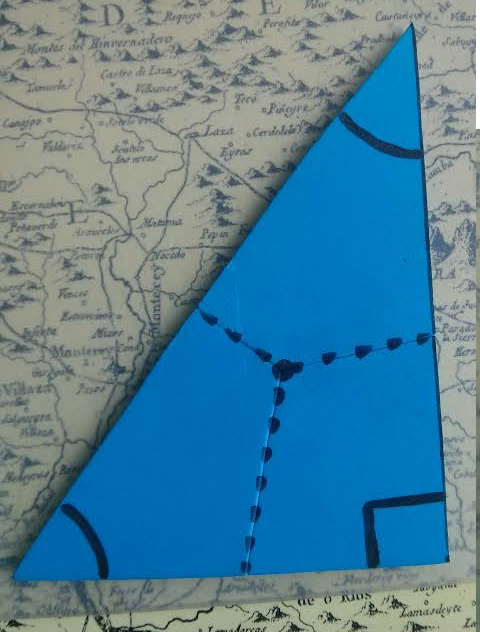
\includegraphics[height=5cm]{img/180grados-2.png}
  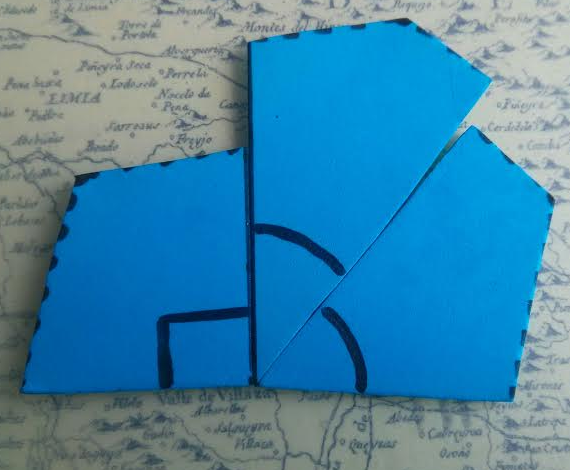
\includegraphics[height=5cm]{img/180grados-1.png}
  \caption{Figuras en goma-eva empregadas para ver a suma dos ángulos dun triángulo}\label{fig:act11}
\end{figure}

\subsubsection{Act. 9: Puntos e rectas notables do triángulo}\label{act9}
Explicamos os puntos e rectas notables recordamos primeiramente as definicións explicadas de mediatriz (como recta cuxos puntos equidistan dos extremos do segmento) e de bisectriz (como recta cuxos puntos equidistan dos lados do ángulo). Unha vez se repasaron estes conceptos, para explicar o circuncentro formulamos un problema no cal deberán buscar a posición ideal para colocar unha antena WiFi que abasteza ao instituto e a un hospital e centro comercial próximos. A formulación do problema acompoñámola coa imaxe que se pode ver na Figura~\ref{fig:act12-1}.

\begin{figure}[h!]
  \centering
  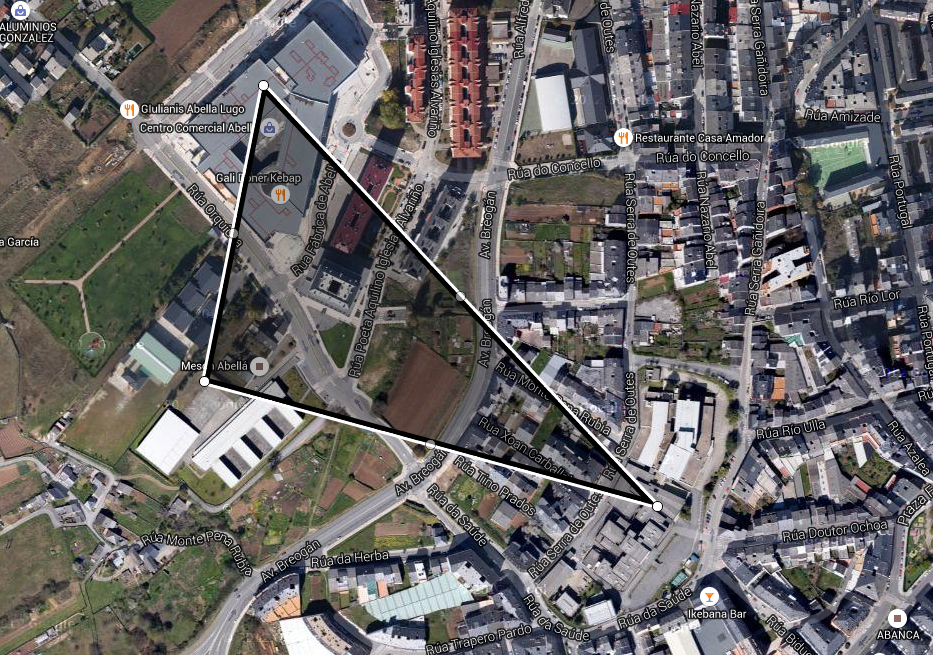
\includegraphics[height=5cm]{img/circuncentro.png}
  \caption{Imaxe empregada para explicar o circuncentro}\label{fig:act12-1}
\end{figure}

Pedimos que o alumnado formule como calcularían este punto e trázanse as solucións empregando o programa Geogebra. Explicamos porque as solucións propostas son ou non correctas e pedindo que expliquen porque a solución correcta consiste en trazar as mediatrices.

\begin{figure}[h!]
  \centering
  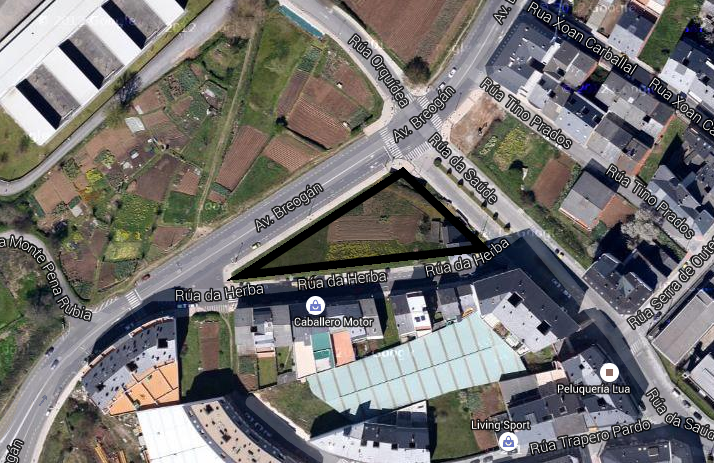
\includegraphics[height=5cm]{img/incentro.png}
  \caption{Imaxe empregada para explicar o incentro}\label{fig:act12-2}
\end{figure}

Para a explicación do dos demais puntos e rectas notables empregáronse métodos similares empregando a imaxe da Figura~\ref{fig:act12-2} para explicar o incentro e pedindo que dividan o triángulo en 6 partes de igual área no caso do baricentro.

\subsubsection{Act. 10: Teorema de Pitágoras}\label{act10}
Explicamos a denominación dos lados dun triángulo rectángulo e a relación entre a lonxitude destes. Relacionamos esta explicación coa area de cadrados con lados a hipotenusa e cada un dos catetos explicando que segundo o teorema cúmprese que a área do cadrado da hipotenusa é igual a suma das áreas dos cadrados dos dous catetos.

\begin{figure}[h!]
  \centering
  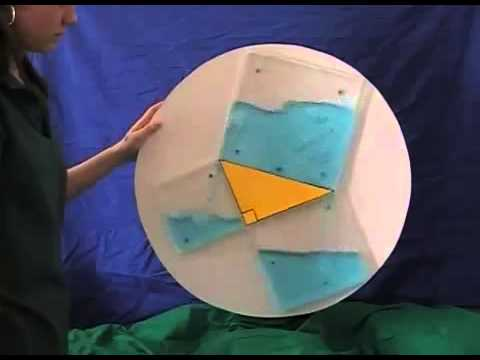
\includegraphics[height=7cm]{img/pitagoras.jpg}
  \caption{Captura dun dos vídeos proxectados con demostracións do Th. de Pitágoras}\label{fig:act10}
\end{figure}

Para reforzar o que explicamos na encerado proxectaremos varios fragmentos do documental \emph{Pitágoras: Mucha más que un teorema}\footnote{Este documental forma parte da serie Universo Matemático feito por RTVE que se pode ver completa en \href{http://www.rtve.es/television/la-aventura-del-saber/documentales/universo-matematico/}{rtve.es/television/la-aventura-del-saber/documentales/universo-matematico}.} relativos aos teorema. Ademais tamén se proxecta unha demostración feita con auga do teorema encontrada nun vídeo en YouTube\footnote{Pódese ver en \href{https://www.youtube.com/watch?v=1er3cHAWwIM}{youtube.com/watch?v=1er3cHAWwIM}.}. A captura da Figura~\ref{fig:act10} pertence a este último vídeo. Despois de ver estas demostracións, faremos exercicios propostos polo libro de texto.

\subsubsection{Act. 11: Clasificación cuadriláteros}\label{act11}
Explicamos a clasificación dos cuadriláteros e a continuación repetimos a mesma actividade que se realizou para practicar a clasificación dos triángulos.  Dividiremos a clase en grupos de 2 ou 3 persoas e cada grupo con un ordenador deberá buscar e marcar 4 cuadriláteros diferentes nas fotos enviadas durante a Actividade 0.
Os alumnos e alumnas enviaran as fotos modificadas ao ordenador do profesor para que estas sexan proxectadas e cada grupo lle poida explicar aos seus compañeiros a clasificación de cada un dos cuadriláteros que marcaron. Na Figura~\ref{fig:act11} pódese ver algún exemplo das figuras que pretendemos acadar.

\begin{figure}[h!]
  \centering
  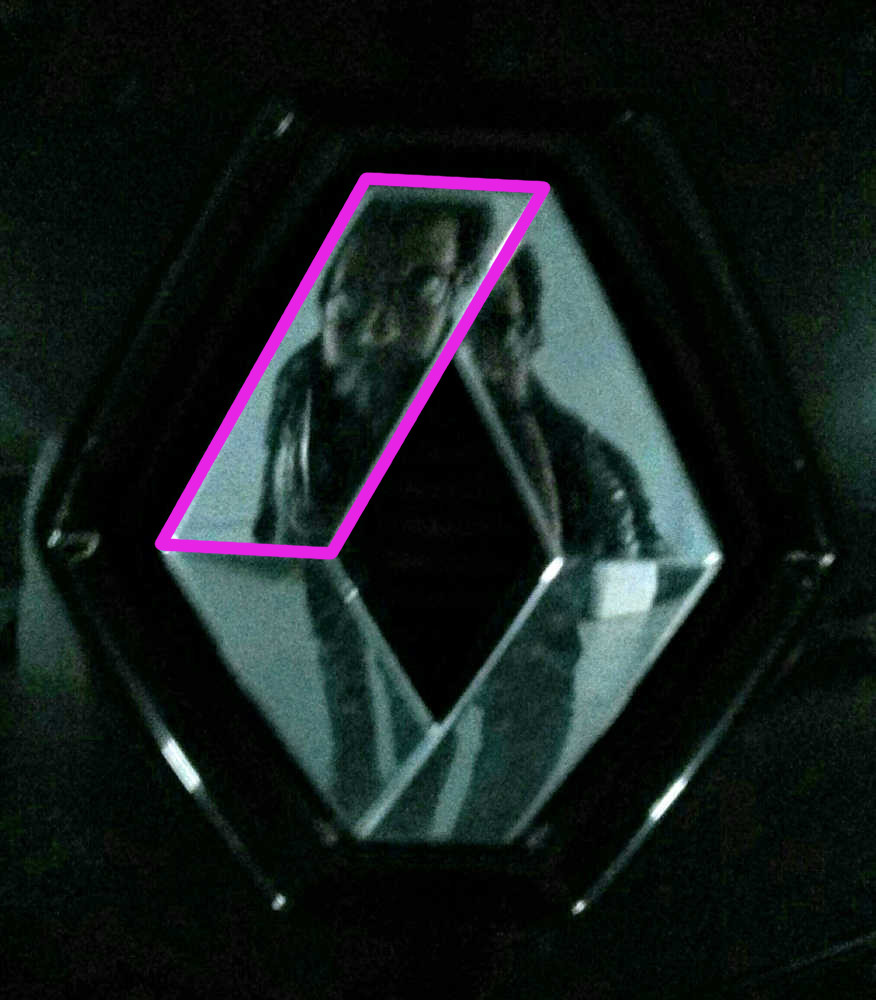
\includegraphics[height=5cm]{img/cuad1.jpg}
  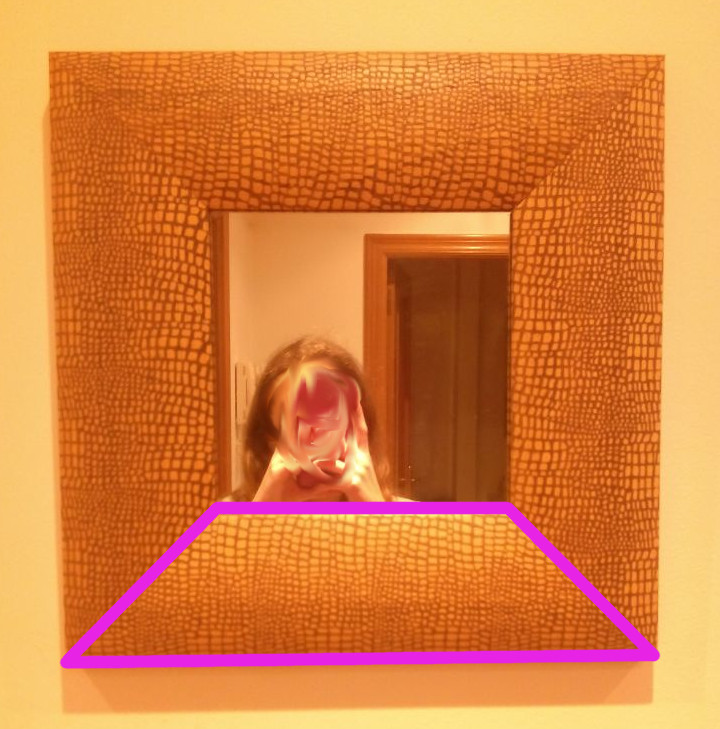
\includegraphics[height=5cm]{img/cuad2.jpg}
  \caption{Exemplo de cuadriláteros marcados sobre as fotografías}\label{fig:act11}
\end{figure}

\subsubsection{Act. 12: Elementos dos polígonos regulares. Circunferencia e círculo} %TODO
Durante esta actividade explicamos algún dos elementos dos polígonos regulares como o radio ou a apotema. Para explicar o concepto de circunferencia pedirémoslles ás alumnas e alumnos que formulen as súas propias definicións para ir corrixíndoas e terminar dando con unha correcta. Explicamos os elementos da circunferencia e por último o círculo e os seus elementos.

\subsubsection{Act. 13: Trivial de Polígonos}\label{act13}
Para practicar todos os conceptos traballados nas leccións anteriores trivial un trivial de 70 preguntas onde se repasan todos estes conceptos. Para facer isto empregamos a plataforma Socrative\footnote{Pódese acceder a ela en \href{http://www.socrative.com/}{socrative.com}.} que dispón dunha aplicativo móbil para a realización dos test así como a súa páxina web. Como se pode ver no Apéndice~\ref{fich:trivial}, as preguntas formuladas eran de varios tipos. Encontramos preguntas onde o alumnado debía seleccionar unha opción entre varias alternativas que lle eran dadas, preguntas onde debían dicir se un enunciado era correcto ou falso e preguntas onde eles mesmos debían escribir a resposta. Na Figura~\ref{fig:act13} pódese ver unha captura de unha posible pregunta que deberían responder as alumnas e alumnos.

\begin{figure}[h!]
  \centering
  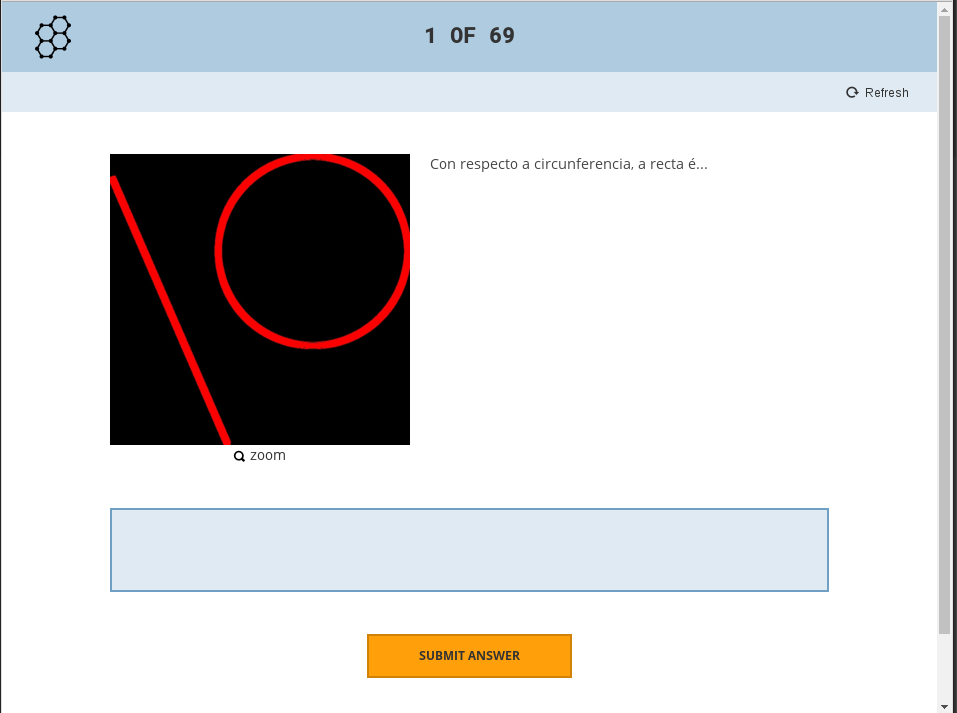
\includegraphics[width=0.8\textwidth]{img/socrative.png}
  \caption{Captura de pantalla dunha pregunta formulada na plataforma Socrative}\label{fig:act13}
\end{figure}

Para a realización do test dividiremos a clase en parellas e cada parella empregará un ordenador. Conectaranse á plataforma de Socrative e responderán a todas as preguntas durante a duración da clase. Durante a sesión seguinte a realización do trivial, analizaremos pregunta a pregunta cal é o resultado correcto e o porqué. Centrarémonos máis nos contidos que fallou a maior parte da clase.

\subsubsection{Act. 14: Exame polígonos}
Realizamos un exame dos contidos traballados anteriormente. O exame pode verse no Apéndice~\ref{fich:ex2}. Da mesma forma que fixemos no primeiro exame, corrixiremos os exames durante esa tarde para amosarllos ao día seguinte corrixidos e que reciban o \emph{feedback} o máis cedo posible.

%TODO: añadir actividade autoevaluación
